%%%%%%%%%%%%%%%%%%%%%%%%%%%%%%%%%%%%%%%%%%%%%%%%%%%%%%%%%%%%%%%%%%%%%%%%%%%%%%%%%%%%%%%%%%%%%%%%%%%%%%%
%%%%%%%%%%%%%% Template de Artigo Adaptado para Trabalho de Diplomação do ICEI %%%%%%%%%%%%%%%%%%%%%%%%
%% codificação UTF-8 - Abntex - Latex -  							     %%
%% Autor:    Fábio Leandro Rodrigues Cordeiro  (fabioleandro@pucminas.br)                            %% 
%% Co-autor: Prof. João Paulo Domingos Silva  e Harison da Silva                                     %%
%% Revisores normas NBR (Padrão PUC Minas): Helenice Rego Cunha e Prof. Theldo Cruz                  %%
%% Versão: 1.0     13 de março 2014                                                                  %%
%%%%%%%%%%%%%%%%%%%%%%%%%%%%%%%%%%%%%%%%%%%%%%%%%%%%%%%%%%%%%%%%%%%%%%%%%%%%%%%%%%%%%%%%%%%%%%%%%%%%%%%
\section{\esp Introdução}

Em um mercado globalizado e competitivo, as tecnologias da informação se tornaram fundamentais para o auxílio da gestão das empresas em suas atividades rotineiras e também no suporte a tomadas de decisões e a possibilidade de desenvolvimento de novos negócios, novos modelos de negócio e a modificação dos valores estratégicos das empresas. \cite{audy}.

Visando a adequação às mudanças mercadológicas, organizacionais e a manutenibilidade em relação a concorrência, o investimento em sistemas de informação tem uma grande parcela do orçamento das empresas, buscando o alinhamento da Tecnologia da informação e negócios. \cite{luftman}  
Para atender a essas necessidades, os requisitos de sistemas têm se tornado cada vez mais complexos, voláteis e robustos diante das demandas das organizações. 
As denominadas metodologias ágeis permitem a entrega de  \textit{software} funcionais em ciclos de desenvolvimento mais curtos considerando a velocidade demandada para a sua construção. \cite{sbbrocco} 
          
No entanto as equipes que lidam com a infraestrutura têm a difícil tarefa de implantar um \textit{software} em produção a medida em que são criados ou modificados, pois estes sistemas requerem dependências de componentes externos, como configurações de \textit{hardware}, sistemas operacionais, banco de dados, servidores de aplicação e web e ainda configurações específicas da aplicação. Isto demanda um tempo considerável para a implantação destes sistemas.

Para garantir um processo totalmente ágil e que acompanhe as exigências do negócio da organização é necessário que haja uma integração do desenvolvimento de sistemas e as operações de infraestrutura. Portanto essa abordagem ágil também deve ser seguida pelas equipes de infraestrutura.
O movimento cultural denominado DevOps surgido em meados de 2009, foi influenciado principalmente por metodologias ágeis e computação na nuvem. Ele teve como fundamento a automatização de processos das operações de infraestrutura e a integração entre as equipes de desenvolvimento e operações. \cite{sato}.

A automatização de processos de infraestrutura é uma das premissas do DevOps, utilizando uma abordagem para provisionar e gerenciar recursos de computação como máquinas virtuais, discos de armazenamento, regras de segurança, instalação de \textit{software}, regras de redes e qualquer outro componente de serviço, destinando-se a simplificar significativamente a configuração e o gerenciamento de recursos em pequena e grande escala. A tradicional administração de um \textit{data center} ou uma nuvem exige que a cada alteração de \textit{software}, uma eventual ação manual na infraestrutura para acertar as configurações. Com a automação a infraestrutura também é tratada como "código" e um desenvolvedor pode descrever os recursos exigidos por uma aplicação em um arquivo padronizado de acordo com a ferramenta utilizada e os \textit{software} de gerenciamento ou provisionamento se encarregará de criar,atualizar ou remover recursos mantendo o estado da infraestrutura. 

\section{\esp Metologia}


\section{\esp Trabalhos Relacionados}


\citeonline{Carnegie} explica que o \textit{design} da infraestrutura é a fase do ciclo de vida do produto em que se define e configura os recursos necessários para o funcionamento dele. A Infraestrutura como código é um conjunto de práticas que usam código para configurar recursos, como máquinas e redes (virtuais), instalar programas, configurar um banco de dados e definir uma regra de segurança. As práticas IaC permitem a criação de vários recursos de maneira automatizada e padronizada, controlando o estado da infraestrutura, além disso permitem o controle de versão, ou seja, pode-se desfazer de qualquer mudança na infraestrutura, somente alterando o código do recursos. Ele também cita que antes mesmo do surgimento da IaC os administradores de sistemas já utilizavam automação, através de \textit{script} para realizar as tarefas de configuração de infraestrutura. E que a IaC surgiu com a popularização da computação da nuvem como serviço e que todos os recursos oferecidos são virtuais. No artigo ele ainda descreve que os provedores de serviços em nuvem fornecem um console de gerenciamento(uma interface \textit{web}) para a administração de recursos. Porém, para um sistema de larga escala, usar o console não é muito prático devido à dificuldade de gerenciar centenas de recursos que são criados e destruídos com uma grande frequência deve-se usar as \textit{application program interface} \footnote{É um conjunto de rotinas e padrões de programação para acesso a um aplicativo de \textit{software} ou plataforma baseada na \textit{Web}, permitindo que dois aplicativos se comuniquem. } (API) disponibilizadas pelo provedor ou Ferramentas IaC  que interagem com essas API que resolvem a questão da criação e destruição de alta frequência desses recursos. Por fim ele cita a relação entre infraestrutura como código \textit{Agile} e o DevOps. 

\hfill

Segundo \citeonline{masek}, a popularização da virtualização e o crescente poder dos servidores e a disponibilidade da computação em nuvem levaram a um aumento significativo no número de servidores e estações de trabalho que precisam ser gerenciados. Nesse ponto, as ferramentas de gerenciamento de orquestração e gerenciamento de configuração se aplicam nesses casos. Os administradores de sistema gerenciam grupos de servidores ou estações de trabalho idênticas (máquinas físicas ou máquinas virtuais) que executam aplicativos e serviços idênticos. Em seu artigo ele apresenta um estudo sobre o uso da ferramenta \textit{Ansible} nos laboratórios da \textit{Brno University of Technology (BUT)}. Ele descreve que o objetivo de utilizar uma ferramenta de IaC é fornecer uma plataforma para gerenciar com eficiência a infraestrutura de larga escala dos laboratórios universitários, com o mínimo de contribuição de desenvolvedores ou administradores.
O autor descreve a infraestrutura como código, como o gerenciamento de redes infraestrutura de trabalho (por exemplo,  em um modelo descritivo. Ele cita dois grupos de ferramentas de infraestrutura como código mais populares: \textit{Chef, Puppet, Ansible e SaltStack}, sendo todas “ferramentas de gerenciamento de configuração”, o que significa que elas foram projetadas para instalar e gerenciar \textit{software} em servidores e estações de trabalho já existentes. E as ferramentas \textit{CloudFormation, Terraform} são “ferramentas de orquestração”, o que significa que eles são projetados para provisionar os servidores.

\hfill

 \citeonline{steve} fala da importância da escolha de ferramentas de IaC como (\textit{ Chef, Ansible, Puppet, SaltStack, Terraform }) se deve levar em consideração o conjunto de casos em que essas ferramentas se propõem a resolver. Estas ferramentas são classificadas em dois domínios: gerenciamento de configurações e orquestração de configuração e quais casos elas resolveram. O autor ainda explica os conceitos de infraestrutura mutável e imutável, escrita de código procedural e declarativa. Este conceitos serão abordados na seção \ref{IaC}. 

\citeonline{steve} expressa que se deve escolher uma ferramenta focada na orquestração de infraestrutura e outra em gerenciamento de configuração de aplicativos reunindo os benefícios de ambas. 

\section{\esp IaC ou Infraestrutura como código} \label{IaC}

Os trabalhos relacionados serviram de base para escrever esta seção. 

\subsection{Gerenciamento de Configuração} 
Ferramentas de gerenciamento de configuração como \textit{Chef, Puppet, Ansible,Saltack} foram projetadas para instalar e gerenciar softwares em servidores já existentes. Por exemplo podendo instalar um banco de dados, adicionar uma regra de \textit{firewall}, realizar uma atualização no sistema operacional. 


\subsection{Provisionamento}

Ferramentas de Provisionamento como \textit{Terraform, Heat, Cloudformation} foram projetadas criar as próprias instâncias \footnote{Uma instância é um servidor virtual na nuvem. Por exemplo: Uma instância rodando o sistema operacional LINUX} e a inicialização de seus recursos. As ferramentas geralmente se concentram no resultado final e ajudam a garantir que o ambiente esteja sempre nesse "estado" 

Segundo \citeonline{Carnegie}, existem sobreposições e esses termos não são mutuamente exclusivos para ambas as ferramentas. As ferramentas de provisionamento podem realizar tarefas de configuração e ferramentas de configuração podem realizar tarefas de provisionamento, porém elas se concentram naquilo que são melhores. 


\subsection{Linguagem}

As ferramentas de IaC usam arquivos de definição como \textit{DSL} 
  \footnote{\textit{DSL - Domain-Specific Language:} Uma linguagem de domínio específico é criada especificamente para resolver problemas em um domínio particular e não se destina a ser capaz de resolver os problemas fora de seu âmbito. }, ou formatos de texto conhecidos comuns como \textit{ YAML} \footnote{\textit{YAML - Ain't  Markup Language}: É um formato de serialização (codificação de dados) de dados legíveis por humanos -  https://yaml.org/ }, \textit{JSON} \footnote{\textit{JSON - JavaScript Object Notation:} É uma formatação leve de troca de dados. Para seres humanos, é fácil de ler e escrever. Para máquinas, é fácil de interpretar e gerar. Está baseado em um subconjunto da linguagem de programação JavaScript, https://www.json.org/json-pt.html}, \textit{XML} \footnote{\textit{XML - eXtensible Markup Language:} é uma linguagem de marcação para a criação de documentos com dados organizados hierarquicamente, tais como textos, banco de dados ou desenhos vetoriais.}
  ou linguagens de programação como \textit{Python} \footnote{\textit{Python} é uma linguagem de programação de alto nível, interpretada, de script, imperativa, orientada a objetos, funcional, de tipagem dinâmica e forte.}  \textit{Ruby} \footnote{\textit{Ruby} é uma linguagem de programação interpretada multi-paradigma, de tipagem dinâmica e forte, com gerenciamento de memória automático.}  ou uma mesclagem de ambas.
 
   \subsubsubsection{Declarativa}
  É o estilo em que você escreve um código que especifica o estado final desejado, e a própria ferramenta IaC é responsável por descobrir como atingir esse estado. Veja o exemplo na Figura \ref{fig:figura2}.
 
 \begin{figure}[ht]
	\centering	
	\caption[\hspace{0.1cm}Exemplo declarativo]{Exemplo de escrita declarativa da ferramenta Terraform}
	\vspace{-0.4cm}
	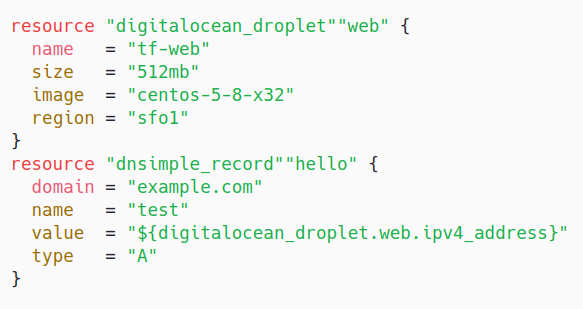
\includegraphics[width=0.5\textwidth]{artigo/figuras/terraform-declarative-exemple-01.png}
	 \vspace{-0.2cm}
	\\\textbf{\footnotesize Fonte: \cite{chef01} }
	\label{fig:figura2}
\end{figure}
\vspace{-0.5cm}
 
 \subsubsubsection{Procedural}
  
  É o estilo na qual você escreve um código e especifica, passo a passo, como atingir o estado final desejado. O ônus recai sobre o usuário para determinar o processo de implantação ideal. Veja o exemplo na Figura \ref{fig:figura1}.

\begin{figure}[ht]
	\centering	
	\caption[\hspace{0.1cm}Exemplo procedural]{Exemplo de escrita procedural da ferramenta Chef}
	\vspace{-0.4cm}
	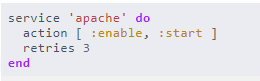
\includegraphics[width=0.5\textwidth]{figuras/chef-io-exemplo-procedural.png}
	 \vspace{-0.2cm}
	\\\textbf{\footnotesize Fonte: \cite{chef01}}
	\label{fig:figura1}
\end{figure}
\vspace{-0.5cm}
  

 \subsection{Infraestrutura}
 
 \subsubsubsection{Mutável}
 Na infraestrutura mutável uma mudança de software será executada nos servidores existentes e com o tempo, à medida em que atualizações são realizadas, cada servidor tem um histórico único de alterações levando erros sutis de configuração. As ferramentas de gerenciamento de configuração, normalmente são padronizadas para um paradigma de infraestrutura mutável.
 
  Um exemplo: Digamos o JAVA precisa ser atualizado. Na infraestrutura mutável cada servidor precisa atualizar a versão do JAVA, geralmente esta atualização pode ser desempenhada por uma ferramenta de gerenciamento de configuração. 
 
 \subsubsubsection{Imutável}
  Segundo \citeonline{Dadgar} A Noção de imutabilidade é a ideia de que, uma vez criada uma coisa, não a mudamos após a criação.
 
 Na infraestrutura imutável qualquer alteração a ser realizada nos servidores eles devem ser recriados. Estas alterações são feitas criando novas configurações e novos servidores são criados a partir delas. Isso aumenta a previsibilidade porque este servidor já foi testado antes de ir para a produção. Em outras palavras, as implantações se tornam atômicas. As ferramentas de provisionamento desempenham este papel.\cite{Morris:2016:ICM:3006361}
 
 Um exemplo: Digamos que precisamos atualizar o \textit{JAVA}\footnote{Java é uma linguagem de programação e plataforma computacional.} para uma versão mais nova. Na infraestrutura imutável é criado um novo servidor com essa atualização. Esta configuração é testada então novos servidores são criados a partir desta configuração e todos que estão rodando a versão antiga do java são destruídos. 
 

\subsection{Arquitetura}

\subsubsubsection{Cliente/Servidor}
 
\subsubsubsection{Cliente} 


\section{Ferramentas}

\subsubsubsection{Ansible}
 
\subsubsubsection{Terraform} 
  
 


 